\begin{figure}[t]
\centering
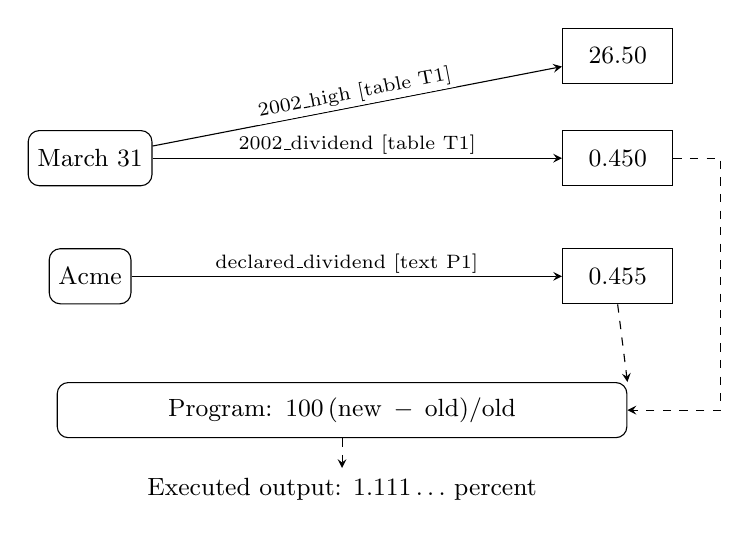
\begin{tikzpicture}[
 entity/.style={draw,rounded corners,align=center,font=\small,minimum height=7mm},
 literal/.style={draw,align=center,font=\small,minimum width=14mm,minimum height=7mm},
 lab/.style={font=\scriptsize,fill=white,inner sep=1pt,align=center},
 flow/.style={->,dashed},>=stealth]
\node[entity] (row) at (0,0) {March 31};
\node[literal] (old) at (6.7,0) {0.450};
\node[literal] (price) at (6.7,1.3) {26.50};
\node[entity] (company) at (0,-1.5) {Acme};
\node[literal] (new) at (6.7,-1.5) {0.455};
\draw[->] (row) -- node[lab,above] {2002\_dividend [table T1]} (old);
\draw[->] (row) -- node[lab,above,sloped] {2002\_high [table T1]} (price);
\draw[->] (company) -- node[lab,above] {declared\_dividend [text P1]} (new);
\node[entity,text width=7cm] (program) at (3.2,-3.2)
 {Program: $100\,(\mathrm{new}-\mathrm{old})/\mathrm{old}$};
\draw[flow] (old.east) -- ++(0.6,0) |- (program.east);
\draw[flow] (new.south) -- (program.north east);
\node[font=\small] (out) at (3.2,-4.2) {Executed output: $1.111\ldots$ percent};
\draw[flow] (program) -- (out);
\end{tikzpicture}
\caption{Illustrative query-time KG and arithmetic data flow. Solid arrows are
stored KG edges, labeled with relation and source identifier. Dashed arrows
are program dependencies, not KG relations. The price edge is a distractor;
only dividend edges supply operands to the displayed computation.}
\label{fig:dividend-kg}
\end{figure}
